\documentclass[a4paper]{article}
\usepackage{geometry}
\geometry{margin=2cm}
\usepackage[T1]{fontenc}
\usepackage{listings}
\usepackage{xcolor}
\usepackage{gensymb}
\usepackage{graphicx}
\usepackage{float}
\definecolor{codegreen}{rgb}{0,0.6,0}
\definecolor{codegray}{rgb}{0.5,0.5,0.5}
\definecolor{codepurple}{rgb}{0.58,0,0.82}
\definecolor{backcolour}{rgb}{0.95,0.95,0.92}

\lstdefinestyle{mystyle}{
    backgroundcolor=\color{backcolour},   
    commentstyle=\color{codegreen},
    keywordstyle=\color{magenta},
    numberstyle=\tiny\color{codegray},
    stringstyle=\color{codepurple},
    basicstyle=\ttfamily\footnotesize,
    breakatwhitespace=false,         
    breaklines=true,                 
    captionpos=b,                    
    keepspaces=true,                 
    numbers=left,                    
    numbersep=5pt,                  
    showspaces=false,                
    showstringspaces=false,
    showtabs=false,                  
    tabsize=4
}

\lstset{style=mystyle}

%opening
\title{Symulator tomografu komputerowego}
\author{Marcin Pastwa 136779\\
Piotr Tomaszewski 136821 }
\date{}


\begin{document}
\maketitle
\section{Zastosowany model tomografu}
Aplikacja symuluje działanie tomografu komputerowego o równoległym modelu układu emiter/detektor.

\section{Zastosowany język programowania oraz dodatkowe biblioteki}
Aplikacja została napisana w języku Python, wykorzystane zostały następujące biblioteki:
\begin{description}
    \item [numpy] Obliczenia macierzowe i wektorowe.
    \item [scikit-image] Odczyt i zapis plików graficznych.
    \item [pydicom] Obsługa plików DICOM.
    \item [tkinter] Interfejs użytkownika.
    \item [pillow] Wyświetlanie obrazów w interfejsie użytkownika.
\end{description}

\section{Opis głównych funkcji progamu}
\subsection{Pozyskiwanie odczytów dla poszczególnych detektorów}
Generowanie sinogramu odbywa się iteracyjnie. W każdej iteracji zmienia się aktualna wartość kąta $\alpha$, zaczynając od wartości 0\degree, kończąc na wartości mniejszej od 180\degree, z krokiem definiowanym przez parametr $\Delta\alpha$. \\
Każda iteracja zaczyna się od wyznaczenia aktualnego położenia emiterów i detektorów. Wartości te są zapisywane, gdyż aplikacja oferuje wizualizację aktualnego stanu skanera.
\begin{lstlisting}[language=Python, caption=Krok transformaty Radona, texcl=true]
def radon_transform_step(self):
    # Wyznaczenie aktualnego położenia emiterów i detektorów
    self.current_emitters, self.current_detectors = \
        self._calculate_emitters_detectors_position()
    # Wyznaczenie linii łączących odpowiadające emitery i detektory
    self.current_scan_lines = \
        self._calculate_scan_lines(self.current_emitters, self.current_detectors)
    self.scan_lines.append(self.current_scan_lines)
    # Wyznaczanie całki po każdej z linii skanera
    for line_id, line in enumerate(self.current_scan_lines):
        line_integral = np.sum([self.input_image[point] for point 
            in self.current_scan_lines[line_id]])
        self.radon_result[line_id, self.current_radon_iteration] += line_integral
    self.current_alpha += self.delta_alpha
    self.current_radon_iteration += 1
\end{lstlisting}
\pagebreak
\begin{lstlisting}[language=Python, caption=Wyznaczanie położenia emiterów i detektorów, texcl=true]
def _calculate_emitters_detectors_position(self):
    emitters = []
    detectors = []
    # Promień obrotu jest połową średnicy okręgu opisanego na obrazie wejściowym
    r = self.circumcircle_diameter // 2
    # Poniżej wyznaczane są kąty $\alpha'$ dla poszczególnych emiterów i detektorów. Gdy wartość kąta $\alpha'$ emitera zmienimy o pewną wartość $x$, a detektora o wartość $-x$, uzyskamy efekt przesunięcia łączącej je linii względem środka okręgu, jednocześnie nie zmieniając nachylenia tej linii
    angles = np.linspace(start=self.current_alpha - self.em_det_spread / 2,
                         stop=self.current_alpha + self.em_det_spread / 2, num=self.em_det_no)
    angles_rad = [math.radians(x) for x in angles]
    for i in range(self.em_det_no):
        angle_rad = angles_rad[i]
        emitter_a = int(self.input_image_center + r * math.cos(angle_rad))
        emitter_b = int(self.input_image_center - r * math.sin(angle_rad))
        emitters.append((emitter_a, emitter_b))
    # Detektory są umieszczane w odwrotnej kolejności. Dzięki temu wszystkie linie łączące odpowiadające sobie emitery i detektory będą (w danej iteracji) tak samo nachylone
    for i in range(self.em_det_no - 1, -1, -1):
        angle_rad = angles_rad[i]
        detector_a = int(self.input_image_center - r * math.cos(angle_rad))
        detector_b = int(self.input_image_center + r * math.sin(angle_rad))
        detectors.append((detector_a, detector_b))
    return emitters, detectors
\end{lstlisting}

\begin{lstlisting}[language=Python, caption=Algorytm Bresenhama, texcl=true]
    def _bresenham(x1, y1, x2, y2):
        delta_x = x2 - x1
        delta_y = y2 - y1
        j = y1
        error = delta_y - delta_x
        points = []
        for i in range(x1, x2 + 1):
            points.append((i, j))
            if error >= 0:
                j += 1
                error -= delta_x
            error += delta_y
        return points
    
    # Poniższa funkcja ma na celu obejście ograniczeń algorytmu Bresenhama, umożliwiając generowanie dowolnych linii
    def generate_line(x1, y1, x2, y2):
        delta_y = abs(y1 - y2)
        delta_x = abs(x1 - x2)
        if delta_y > delta_x:
            points = generate_line(y1, x1, y2, x2)
            for i in range(len(points)):
                points[i] = (points[i][1], points[i][0])
        elif y2 < y1 and x2 < x1:
            points = _bresenham(x1, y1, x1 + delta_x, y1 + delta_y)
            for i in range(len(points)):
                points[i] = (2 * x1 - points[i][0], 2 * y1 - points[i][1])
        elif y2 < y1:
            points = _bresenham(x1, y1, x2, y1 + delta_y)
            for i in range(len(points)):
                points[i] = (points[i][0], 2 * y1 - points[i][1])
        elif x2 < x1:
            points = _bresenham(x1, y1, x1 + delta_x, y2)
            for i in range(len(points)):
                points[i] = (2 * x1 - points[i][0], points[i][1])
        else:
            points = _bresenham(x1, y1, x2, y2)
        return points
    \end{lstlisting}
\pagebreak
\subsection{Ustalanie jasności poszczególnych punktów obrazu wynikowego\\ oraz jego przetwarzanie końcowe}
Odtwarzanie obrazu wygląda bardzo podobnie do generowania sinogramu. Jednak, zamiast wyznaczać całkę po kolejnych liniach skanujących, dodajemy jej wartość do każdego piksela obrazu wynikowego, który do tej linii należy.
\begin{lstlisting}[language=Python, caption=Krok odtwarzania obrazu, texcl=true]
def iradon_step(self):
    for s, line in enumerate(self.scan_lines[self.current_iradon_iteration]):
        for point in line:
            self.iradon_result[point] += self.radon_result[s, self.current_iradon_iteration]
    self.current_iradon_iteration += 1
\end{lstlisting}
Następnie, wynikowy obraz zostaje poddany normalizacji. Przyjęliśmy, że pracujemy z obrazami 8-bitowymi.
\begin{lstlisting}[language=Python, caption=Normalizacja odtworzonego obrazu, texcl=true]
def visualize_reconstructed_img(self):
    # Usunięcie poprzedniego obrazu, jeśli taki istnieje
    self.rec_img = np.zeros((self.iradon_result.shape[0], self.iradon_result.shape[1]), dtype=np.uint8)
    max_val = np.max(self.iradon_result)
    min_val = np.min(self.iradon_result)
    for i in range(len(self.iradon_result)):
        for j in range(len(self.iradon_result[i])):
            self.rec_img[i, j] = \
                int((self.iradon_result[i, j] - min_val) / (max_val - min_val) * 255)
    return self.rec_img
\end{lstlisting}

\subsection{Odczyt i zapis plików DICOM}
Aplikacja wspiera obsługę plików DICOM. Mimo, że pliki te, z zasady, przechowują wynik badania tomografem, tj. już odtworzony obraz, uznaliśmy że może on posłużyć za dane wejściowe naszego symulatora.\\
Program umożliwia odczyt i zapis podstawowych informacji o badaniu i pacjencie, komentarza i obrazu w formacie DICOM.
\begin{lstlisting}[language=Python, caption=Wczytywanie plików DICOM, texcl=true]
def dicom_load(path):
    # zbiór danych DICOM
    ds = pydicom.dcmread(path)
    image = ds.pixel_array
    # Przyjęliśmy, że pracujemy z obrazami 8-bitowymi
    if image.dtype != np.uint8:
        img_max = np.max(image)
        img_min = np.min(image)
        image = 255 * (image - img_min) / (img_max - img_min)
    return ds, image.astype(np.uint8)
\end{lstlisting}
Aby ułatwić dalszą pracę i zwiększyć czytelność danych pozyskanych z pliku DICOM, interesujące nas pola zostają odpowiednio sformatowane i umieszczone w słowniku \texttt{data}. \\
Zbiór danych \texttt{dataset} jest obiektem dostarczanym przez bibiliotekę \textit{pydicom}, który przechowuje w swojej strukturze poszczególne pola zdefiniowane w standardzie DICOM.
\begin{lstlisting}[language=Python, caption=Odczyt interesujących wartości ze zbioru danych DICOM, texcl=true]
def dicom_read_dataset(dataset):
    data = {}
    if dataset.get('StudyDate'):
        data['StudyDate'] = dicom_date_dataset_to_display(dataset.get('StudyDate'))
    else:
        data['StudyDate'] = ''
    if dataset.get('StudyTime'):
        data['StudyTime'] = dicom_time_dataset_to_display(dataset.get('StudyTime'))
    else:
        data['StudyTime'] = ''
    data['PatientID'] = str(dataset.get('PatientID') or '')
    if dataset.get('PatientName'):
        patient_name = dataset.get('PatientName')
        try:
            data['PatientGivenName'] = patient_name.given_name
        except AttributeError:
            data['PatientGivenName'] = ''
        try:
            data['PatientFamilyName'] = patient_name.family_name
        except AttributeError:
            data['PatientFamilyName'] = ''
    else:
        data['PatientGivenName'] = ''
        data['PatientFamilyName'] = ''
    sex = dataset.get('PatientSex')
    if sex:
        if sex == 'F':
            data['PatientSex'] = 'Kobieta'
        elif sex == 'M':
            data['PatientSex'] = 'Mezczyzna'
    else:
        data['PatientSex'] = 'Nieznana'
    bday = dataset.get('PatientBirthDate')
    if bday:
        data['PatientBirthDate'] = dicom_date_dataset_to_display(bday)
    else:
        data['PatientBirthDate'] = ''
    data['ImageComments'] = dataset.get('ImageComments') or ''
    return data
\end{lstlisting}
Jeżeli użytkownik otworzy obraz wejściowy, który nie jest plikiem DICOM, zostaje utworzony i zainicjalizowany nowy zbiór danych, który jest następnie umieszczany w pliku tymczasowym.
\begin{lstlisting}[language=Python, caption=Tworzenie nowego pliku DICOM, texcl=true]
def dicom_create_new_dataset():
    suffix = '.dcm'
    file_name = tempfile.NamedTemporaryFile(suffix=suffix).name
    file_meta = Dataset()
    # Ustawienie niektórych wymaganych wartości (pozostałe ustawiane przy zapisie)
    file_meta.MediaStorageSOPClassUID = '1.2.840.10008.5.1.4.1.1.2'
    file_meta.MediaStorageSOPInstanceUID = "1.3.6.1.4.1.5962.1.1.1.1.1.20040119072730.12322"
    file_meta.ImplementationClassUID = "1.3.6.1.4.1.5962.2"
    file_meta.TransferSyntaxUID = '1.2.840.10008.1.2'
    return FileDataset(file_name, {}, file_meta=file_meta, preamble=b"\0" * 128)
\end{lstlisting}
Po zatwierdzeniu przez użytkownika wprowadzenia danych o badaniu i pacjencie oraz komentarza, zostają one sformatowane tak, aby spełniać warunki standardu DICOM, a następnie są zapisywane do przechowywanego w pamięci zbioru danych.
\begin{lstlisting}[language=Python, caption=Wpisywanie danych do zbioru danych DICOM]
def dicom_store_data(data, dataset):
    if data.get('StudyDate'):
        dataset.StudyDate = dicom_date_display_to_dataset(data.get('StudyDate'))
    if data.get('StudyTime'):
        dataset.StudyTime = dicom_time_display_to_dataset(data.get('StudyTime'))
    if data.get('PatientGivenName') or data.get('PatientFamilyName'):
        patient_given_name = data.get('PatientGivenName') or ''
        patient_family_name = data.get('PatientFamilyName') or ''
        dataset.PatientName = '^'.join((patient_family_name, patient_given_name))
    if data.get('PatientID'):
        dataset.PatientID = data.get('PatientID')
    if data.get('PatientSex'):
        if data.get('PatientSex') == 'Mezczyzna':
            dataset.PatientSex = 'M'
        elif data.get('PatientSex') == 'Kobieta':
            dataset.PatientSex = 'F'
    if data.get('PatientBirthDate'):
        dataset.PatientBirthDate = dicom_date_display_to_dataset(data.get('PatientBirthDate'))
    if data.get('ImageComments'):
        dataset.ImageComments = data.get('ImageComments')
    return dataset
\end{lstlisting}
\pagebreak
Użytkownik posiada wybór, czy umieścić w pliku DICOM obraz wyjściowy, czy też wejściowy. Ta druga opcja może być przydatna, gdy ma on zamiar jedynie uzupełnić dane w już istniejącym pliku.
\begin{lstlisting}[language=Python, caption=Zapis pliku DICOM, texcl=true]
def dicom_save(file_name, dataset, image):
    # Upewnienie się, że wyjściowy obraz ma właściwy format
    if image.dtype != np.uint8:
        img_max = np.max(image)
        img_min = np.min(image)
        image = ((image - img_min) / (img_max - img_min) * 255)
        image = image.astype(np.uint8)
    dataset.SpecificCharacterSet = 'utf-8'
    # Konwersja obrazu i ustawienie jego parametrów
    dataset.PixelData = image.tobytes()
    dataset.Rows, dataset.Columns = image.shape
    dataset.BitsStored = 8
    dataset.BitsAllocated = 8
    dataset.HighBit = 7
    dataset.SamplesPerPixel = 1
    dataset.PhotometricInterpretation = "MONOCHROME2"
    dataset.PixelRepresentation = 0
    dataset.save_as(file_name, write_like_original=False)
    \end{lstlisting}
\section{Wygląd aplikacji}
\begin{figure}[H]
\center{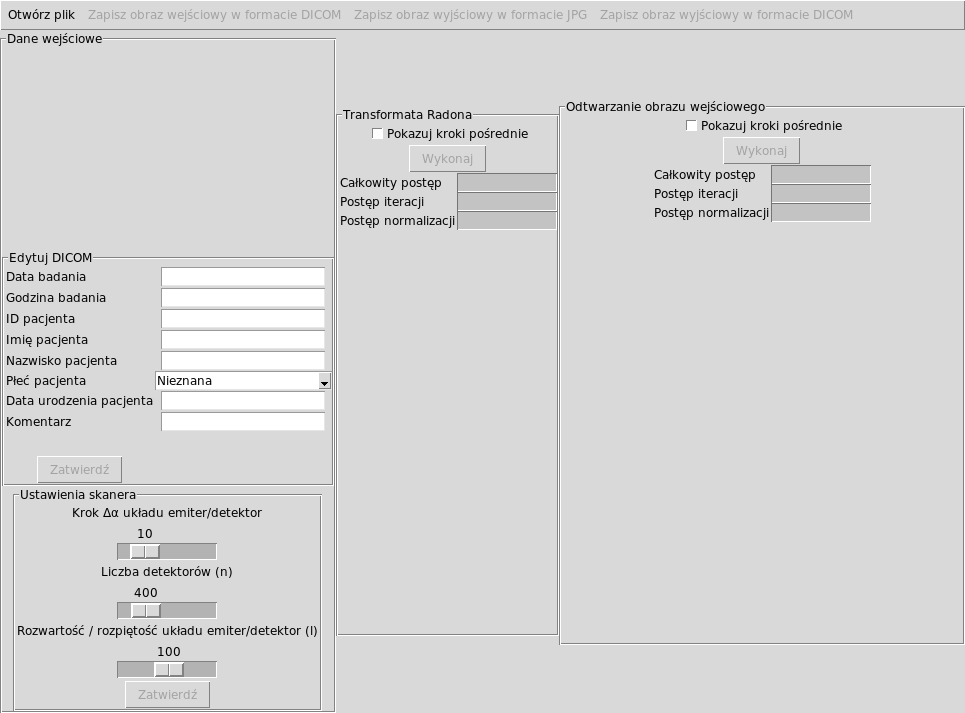
\includegraphics[width=0.8\linewidth]{pic/app.png}}
\caption{Ekran aplikacji}
\end{figure}
\begin{figure}[H]
\center{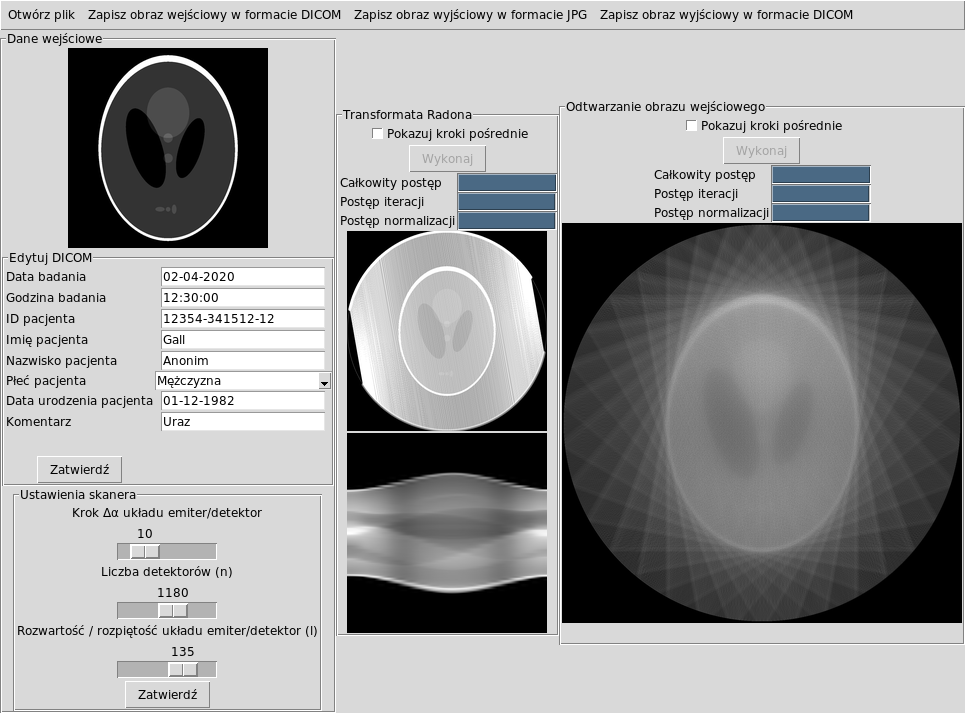
\includegraphics[width=0.8\linewidth]{pic/result.png}}
\caption{Przykład działania}
\end{figure}
\section{Sprawdzenie poprawności pliku DICOM}
Poprawność tworzonych plików DICOM weryfikowana była za pomocą \\ \texttt{https://www.ofoct.com/viewer/dicom-viewer-online.html}
\begin{figure}[H]
    \center{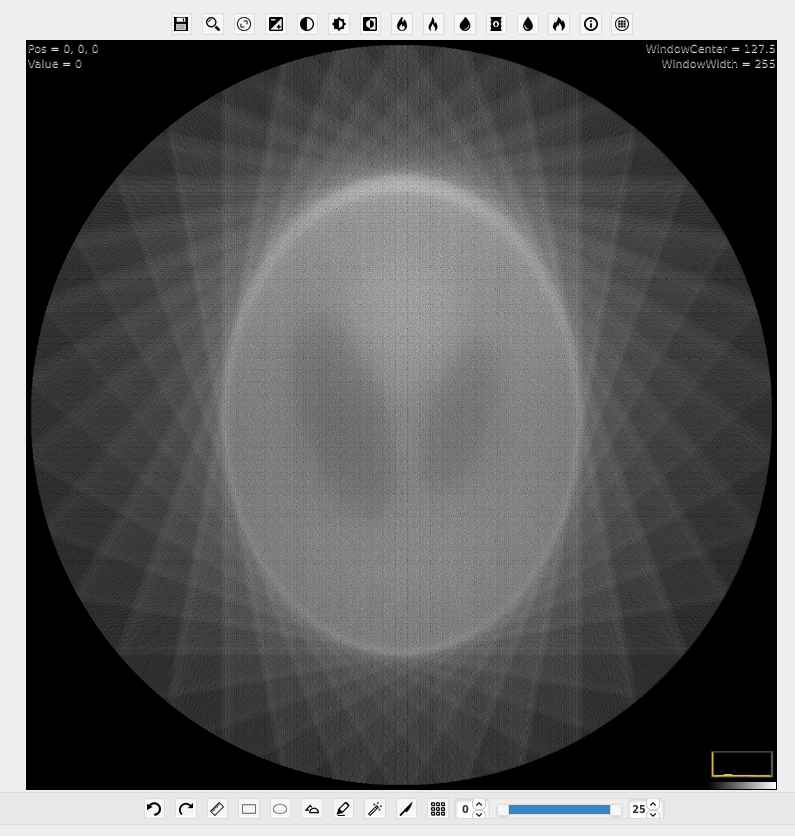
\includegraphics[width=0.5\linewidth]{pic/check_img.png}}
    \caption{Weryfikacja poprawności obrazu}
\end{figure}
\begin{figure}[H]
    \center{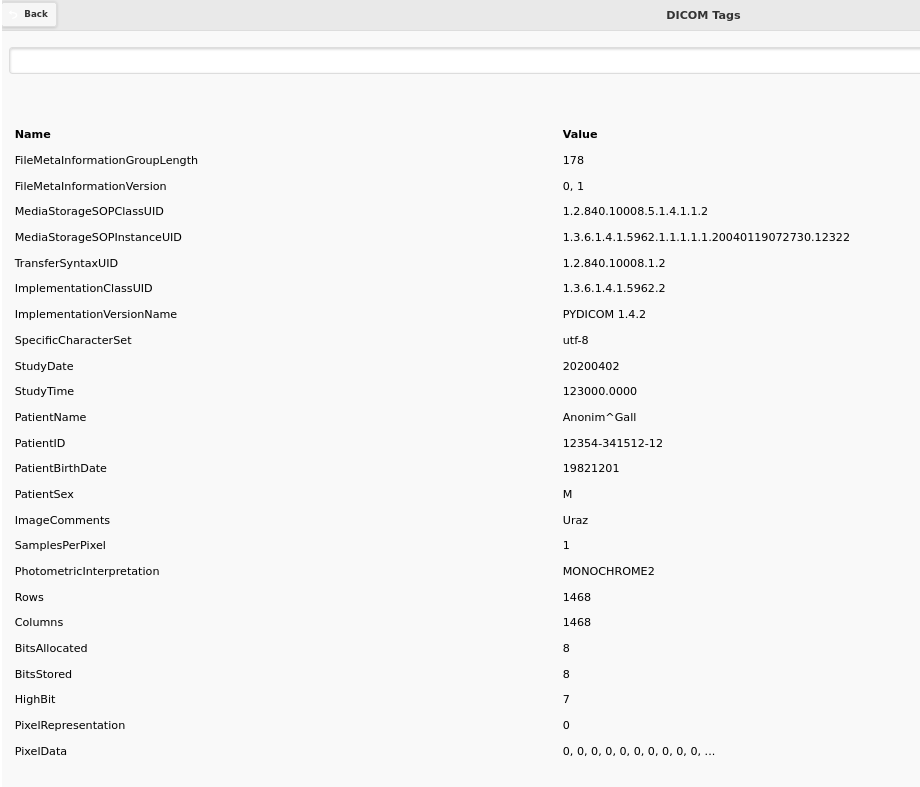
\includegraphics[width=0.8\linewidth]{pic/check_tags.png}}
    \caption{Weryfikacja poprawności tagów}
\end{figure}
\end{document}
